\begin{longtable} { | c | p{12cm} | c | } 
\hline
	ID 	&	Issues	&		 Es. hours \\\hline
	50 	&	Sequenceviewer: an arrow highlighting method	&	16 hours \\\hline
\caption{Issue ID 50}
\label{tab:spr3_SVarrowhighlight}
\end{longtable}

As stated in appendix \ref{app:reqgroup1}, it is required that the users can mark how far they are in a sequence. This has been implemented by setting up a picture of an arrow, which are placed above the first pictogram in a sequence.

In the landscape$\_$mode.xml file, an ImageView with the picture of an arrow as background is created. It is located in a LinearLayout which is placed in the hierarchy at same level as the ScrollView. The ImageView has its visibility set to \textit{invisible}. This can be seen in listing \ref{lst:arrowXML}.

\begin{lstlisting} [caption={A section of the xml-code in landscape$\_$mode}, label={lst:arrowXML}]
        <LinearLayout
            android:id="@+id/land_arrow_linlay"
            android:orientation="horizontal"
            android:layout_width="wrap_content"
            android:layout_height="wrap_content">

                <ImageView
                android:id="@+id/arrow"
                android:layout_width="match_parent"
                android:layout_height="match_parent"
                android:background="@drawable/arrowtemp"
                android:visibility="invisible"/>
                
        </LinearLayout>
\end{lstlisting}

We have then created a method in the HorizontallyScroll class called \ct{setupMarker}. This method aligns the marker above the first pictogram in the sequence, and sets its visibility to \textit{visible}. The alignment is done by first targetting the LinearLayout which contains the ImageView with the arrow. We then assign as much space as a pictogram for width and wrap$\_$content for height, and define these as the layout-parameters for this LinearLayout.

We then add alignment rules for the LinearLayout, this is done because it is placed inside a RelativeLayout. We use \ct{ALIGN$\_$LEFT, mainLayout.getChildAt(0).getId()} and \newline \ct{ABOVE, mainLayout.getChildAt(0).getId()}, to make the arrow stay above the first pictogram in the sequence. Last we center everything inside the LinearLayout.

We set the arrow to \textit{visible}, and tell the ScrollView to stay below the arrow with \ct{BELOW, arrow$\_$linlay.getId()}. The code can be seen in \ref{lst:markerMethod}.

\begin{lstlisting} [caption={Method for setting up the marker}, label={lst:markerMethod}]
    private void setupMarker(){

        arrow_linlay = (LinearLayout) landscape.findViewById(R.id.land_arrow_linlay);
        RelativeLayout.LayoutParams myParams = new RelativeLayout.LayoutParams(getWidth() / numberOfVisibiblePictograms, LinearLayout.LayoutParams.WRAP_CONTENT);
        myParams.addRule(RelativeLayout.ALIGN_LEFT, mainLayout.getChildAt(0).getId());
        myParams.addRule(RelativeLayout.ABOVE, mainLayout.getChildAt(0).getId());
        arrow_linlay.setGravity(Gravity.CENTER);
        arrow_linlay.setLayoutParams(myParams);


        ImageView arrow = (ImageView) landscape.findViewById(R.id.arrow);
        arrow.setVisibility(VISIBLE);
        arrow.setTag("This_is_an_arrow_marker");

        RelativeLayout.LayoutParams myMain = (RelativeLayout.LayoutParams)this.getLayoutParams();
        myMain.addRule(RelativeLayout.BELOW, arrow_linlay.getId());
        this.setLayoutParams(myMain);

    }
\end{lstlisting}

The marker can be seen attached to a five pictogram long sequence shown in figure \ref{fig:markerpic}, which is displayed in landscape-mode.
\begin{figure} [h!]
\centering
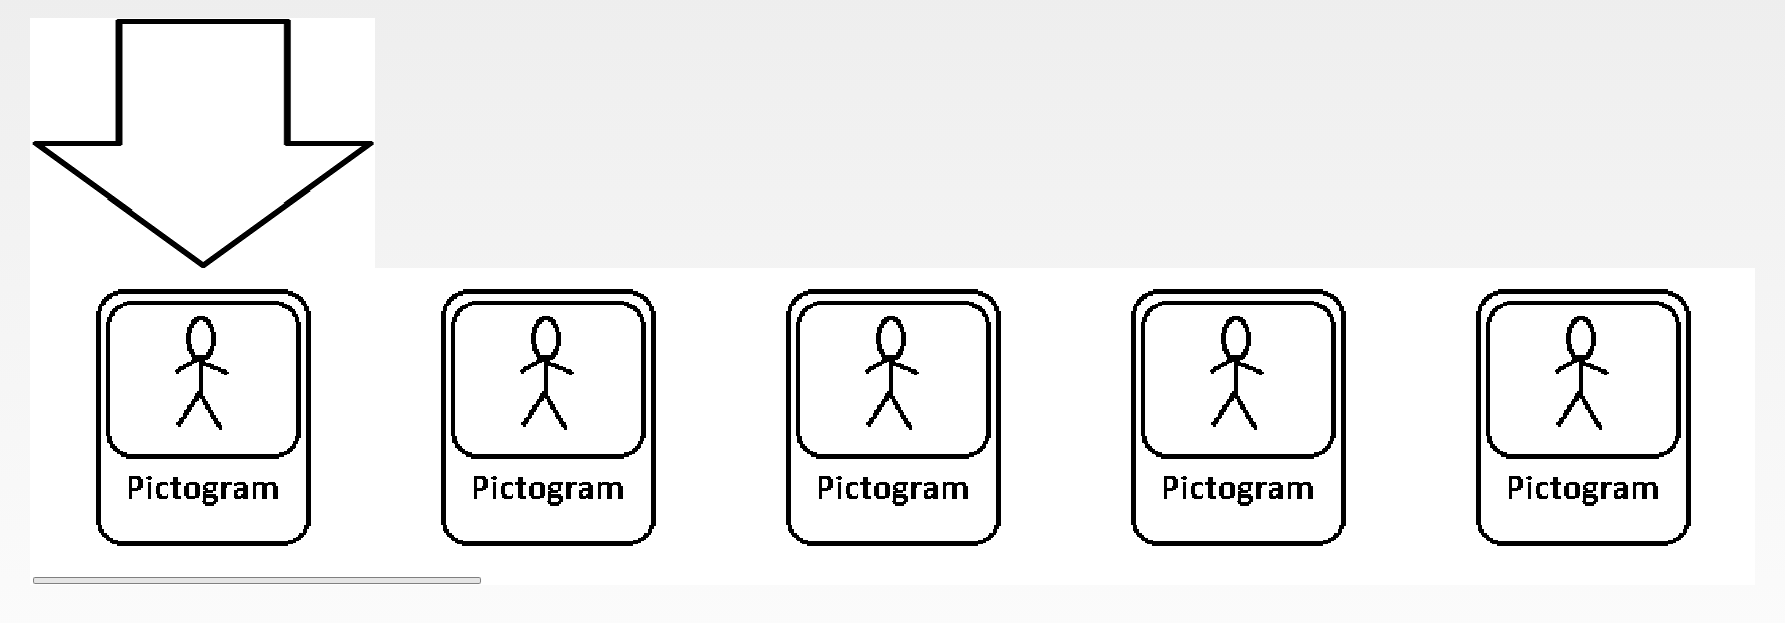
\includegraphics[width=0.9\textwidth]{Pics/Sprint3/landscape5picsCROP.png}
\caption{This is the arrow-marker displayed above the first pictogram in a sequence displayed in landscape-mode}
\label{fig:markerpic}
\end{figure}